\documentclass{standalone}
\usepackage{tkz-fct}
\usepackage{tkz-euclide}
\usepackage{color}
\renewcommand*\familydefault{\sfdefault}
\usepackage{sansmath}
\sansmath
\definecolor{gray75}{gray}{0.75}
\begin{document}
 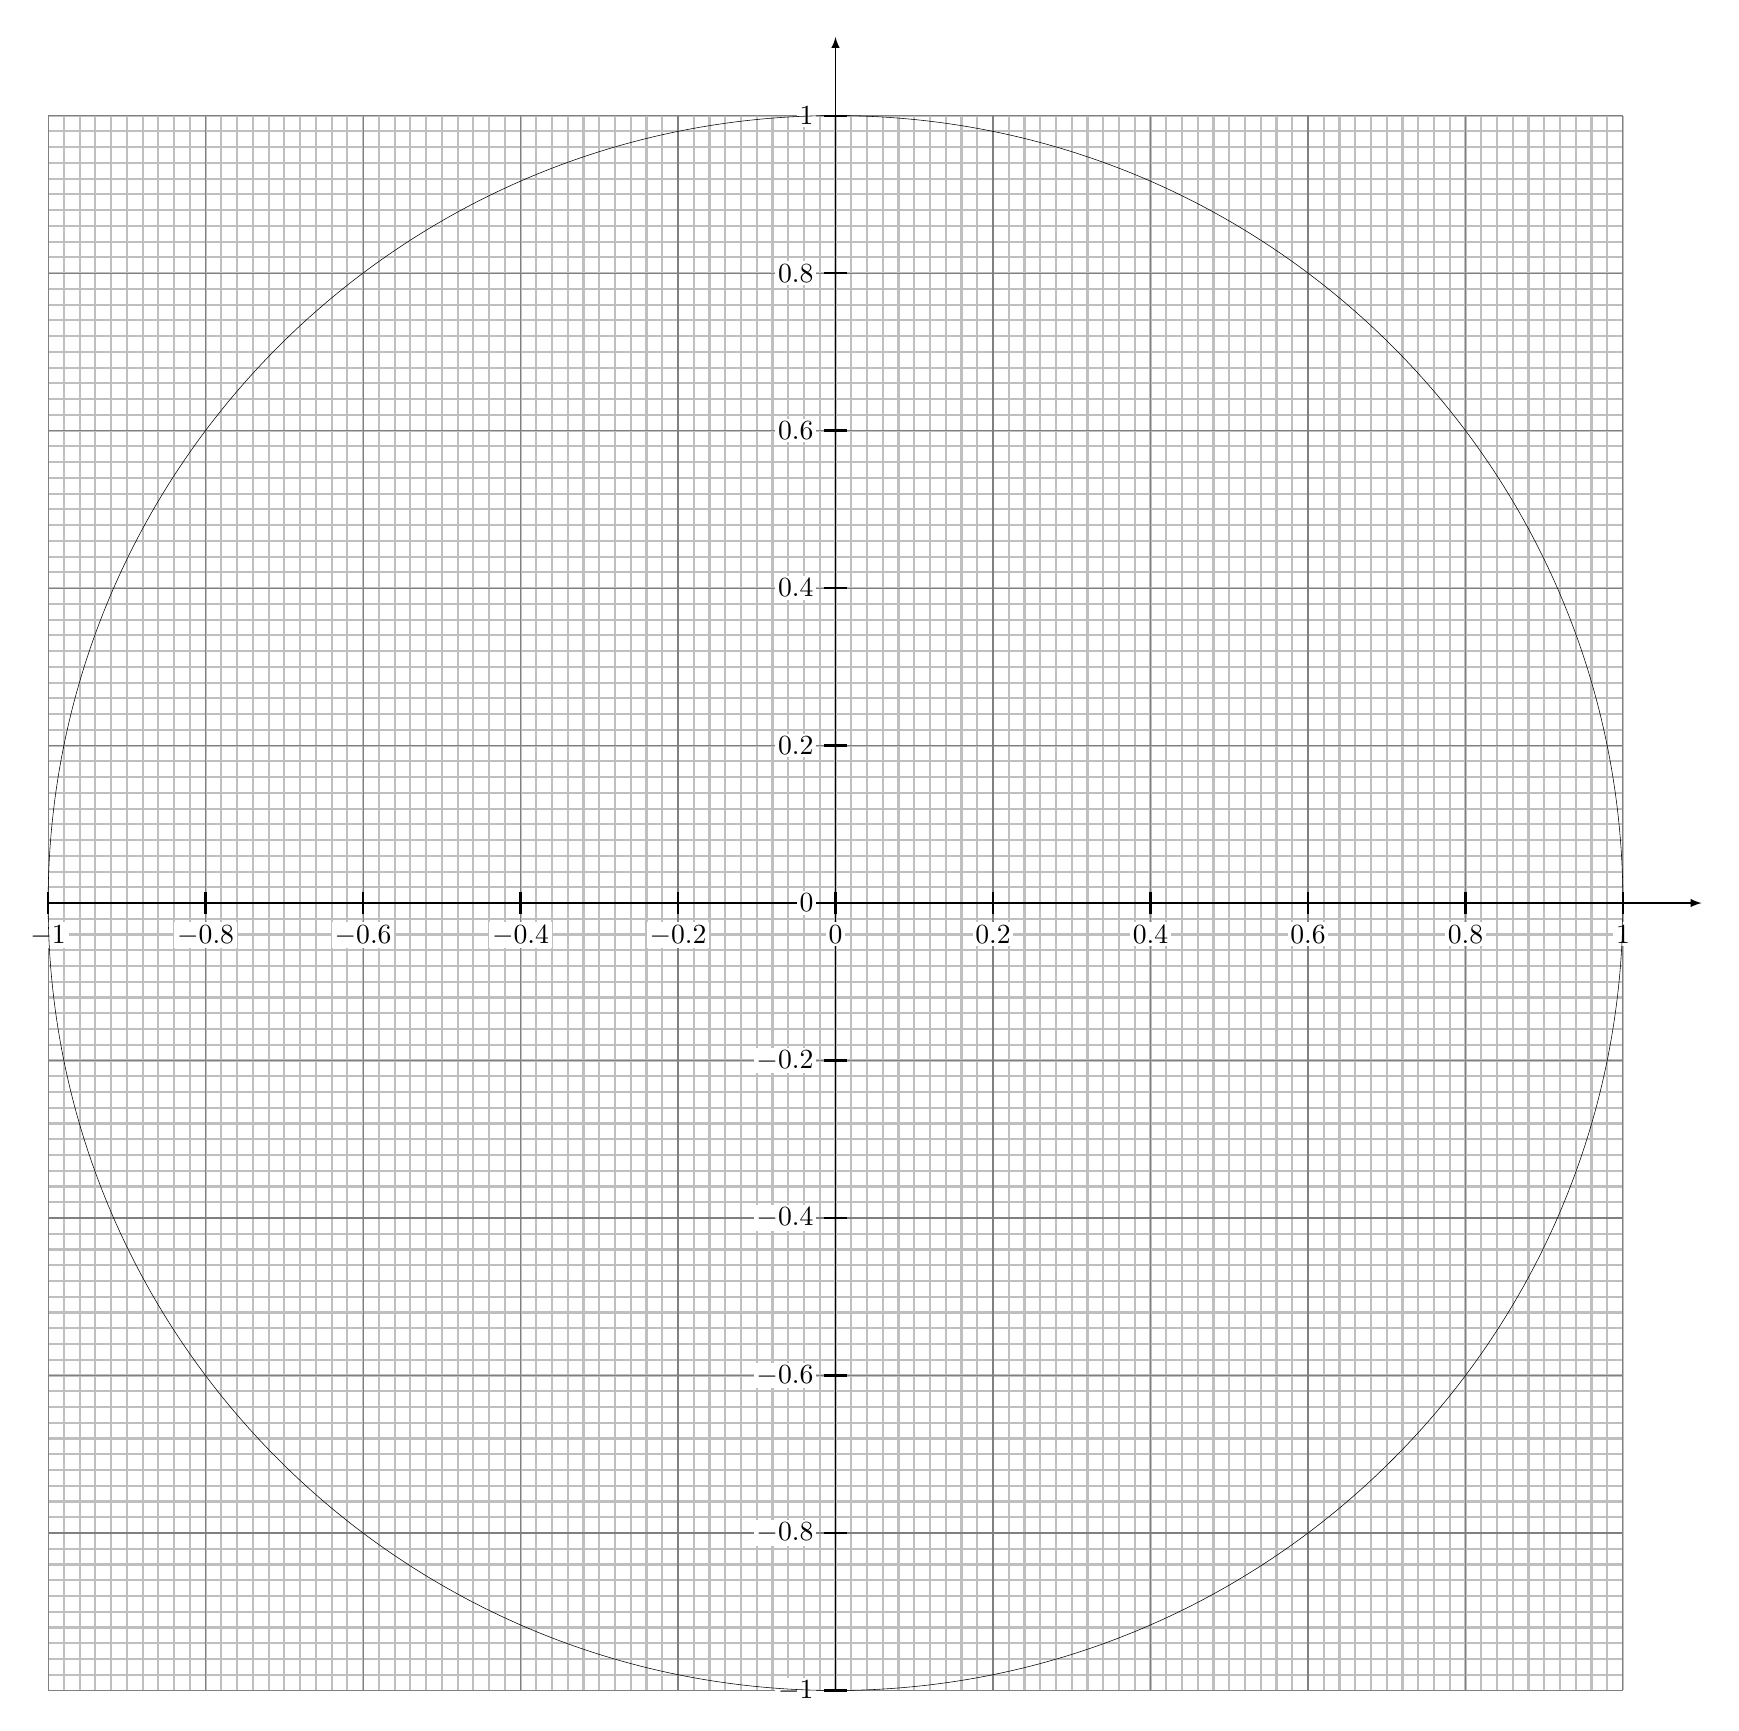
\begin{tikzpicture}[scale=2]
   \tkzInit[xmax=1.,ymax=1.,xmin=-1. ,ymin=-1,xstep=0.2,ystep=0.2]
   
   \begin{scope}
     \tkzGrid[sub,subxstep=0.02,subystep=0.02]
   \end{scope}
   \tkzAxeXY[label={}]
   \tkzDefPoints{0/0/O,1/0/A}
   \tkzDrawCircle[color=black](O,A)


\end{tikzpicture}
\end{document}
